% !TeX root = ../thesis_main.tex

% ---------------------------------------------------
% ----- Chapters of the template
% ----- for Bachelor-, Master thesis and class papers
% ---------------------------------------------------
%  Created by C. Müller-Birn on 2012-08-17, CC-BY-SA 3.0.
%  Freie Universität Berlin, Institute of Computer Science, Human Centered Computing. 
%
\chapter{Prototyping}
\label{chap:prototyping} 

After collecting the initial user feedback, minimal digital ``paper'' prototypes were created using Figma\footnote{Figma (\url{https://www.figma.com/}) is a design tool accessible through the browser for collaborative work on design projects.} to gather visualizations of the proposed UI layouts.
Two ideas emerged from the interviews: a (file-)editor-centric layout and a preview-centric layout.
\section{Editor centric vs. preview centric layout}

The \textbf{preview-centric layout} is inspired by popular generic website builders like \url{https://wix.com} or \url{https://wordpress.com}, where the user
can see the page in an interactive mode, move, configure or place elements, and then has on the side additional panels like one with information \& options about the
currently selected element.
There are also framework-agnostic tools like \url{https://vwo.com/why-us/technology/visual-editor/}, but they either focused more on only editing the style and not the structure of the page or were not
compatible with the Experience's framework and data format. 
\begin{figure}[h!]
  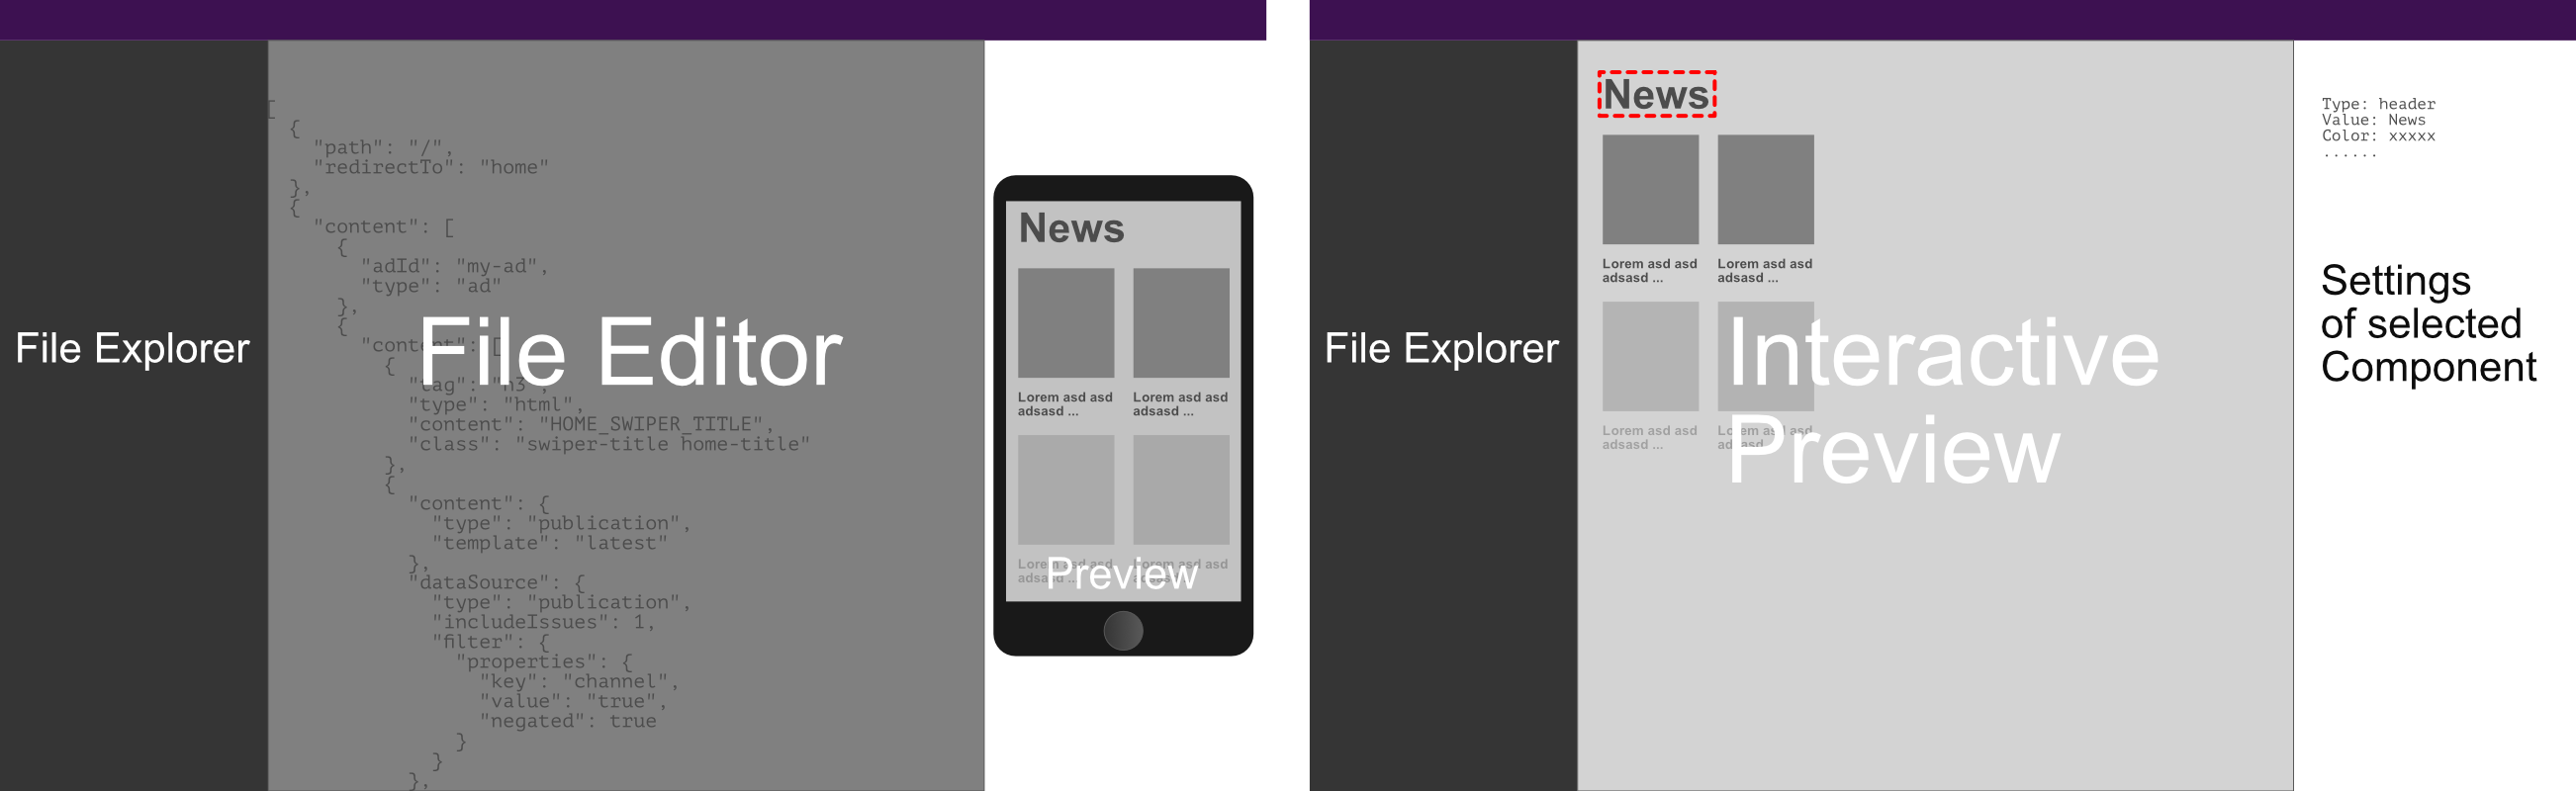
\includegraphics[width=\textwidth]{pics/editor_centric_vs_preview_centric.png}
  \caption{Mockups: Editor centric vs preview centric editor layout}
\end{figure}
\newpage
The \textbf{editor-centric layout} is inspired by modern text editors / \Gls{ide}s like VS Code (\url{https://code.visualstudio.com/}), which was mentioned as reference during the interviews multiple times.
There, the central pane is the editor for the currently open file, while on the sides additional panes for file management, preview and more can be shown.
The familiarity, especially to developers who are used to IDE layouts, could help new users adopt patterns to work with the UI they use in other tools as well.
\begin{figure}[h!]
  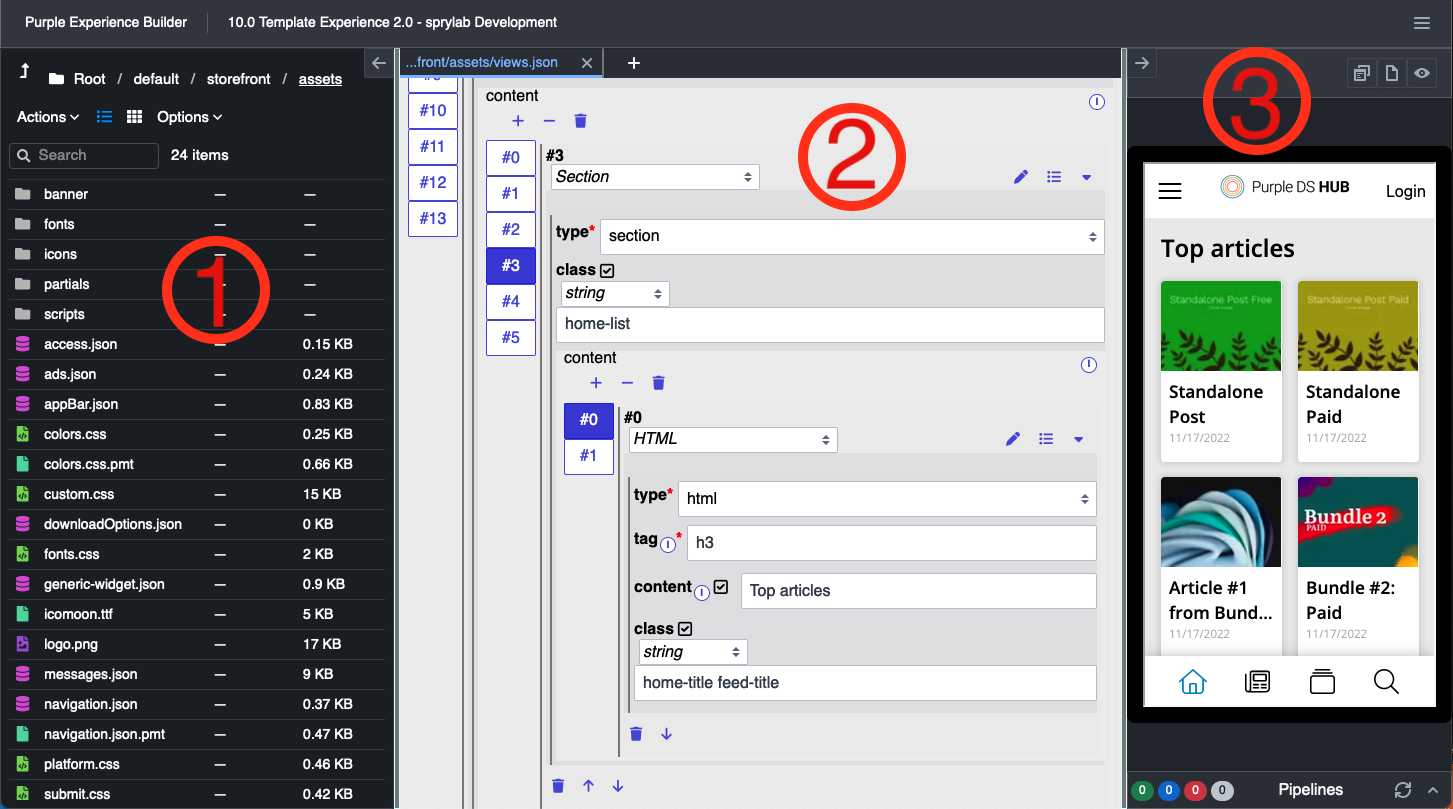
\includegraphics[width=\textwidth]{pics/editor-centric-screenshot.png}
  \caption{Editor centric todo}
  \label{fig:editor-centric}
\end{figure}
\bigskip
Here are some reasons why the editor centric layout was chosen and not the preview-centric one:
\begin{itemize}
  \item The configuration structure of the \Gls{experience} framework was not built with preview-based editing in mind, causing many functionalities to be hidden and invisible to the user, making it difficult to reproduce specific conditions in the editor environment.
  Thus, editing in a preview-centric mode could lead to more confusion for the editors than speeding up the process.
  As the configuration schemata are mostly fixed, it was deemed that preview-based editing would not be suitable in this case.
  \item After evaluating available libraries and examples, we concluded that building a reliable and usable preview-centric editor is more complicated and uncertain to result in a viable product within the limited time frame of this bachelor thesis.
  For editor-centric UIs, many third-party libraries exist that can be integrated into the UI, such as Microsoft's Monaco Editor (\url{https://microsoft.github.io/monaco-editor/}) for editing generic web-related files with automatic syntax highlighting and error detection, and JSON Editor for working with JSON configurations with provided schema.
  \item The user base consists mostly of tech-affine people who are used to layouts of IDEs, and the old tool also had a similar editor-centric layout.
  As Jakob's Law of the Internet User Experience states, the user's understanding of a website is directly tied to their mental model of that system \cite{Nielsen:2000} and \cite[p. 2]{LawsOfUX:2020ys}. Introducing an unconventional workflow comes with the danger of confusing the user, causing mistakes, and potentially leading to dissatisfaction with the tool.
 
\end{itemize}

